\documentclass[tikz,border=10pt]{standalone}
\usepackage{tikz}
\usepackage{fontawesome5}
\usepackage{amsmath,amssymb}
\usetikzlibrary{arrows.meta,positioning,fit,backgrounds,calc,shadows,shapes.geometric}

\definecolor{civNavy}{RGB}{15, 34, 64}
\definecolor{civBlue}{RGB}{28, 80, 160}
\definecolor{civTeal}{RGB}{14, 130, 120}
\definecolor{civLightBlue}{RGB}{238, 245, 255}
\definecolor{civBorder}{RGB}{185, 210, 240}
\definecolor{civGold}{RGB}{217, 119, 6}
\definecolor{civGreen}{RGB}{22, 130, 80}
\definecolor{civDark}{RGB}{20, 28, 42}
\definecolor{cInput}{RGB}{240, 246, 255}
\definecolor{cStem}{RGB}{224, 242, 254}
\definecolor{cStage1}{RGB}{209, 250, 229}
\definecolor{cStage2}{RGB}{254, 243, 199}
\definecolor{cStage3}{RGB}{254, 226, 226}
\definecolor{cStage4}{RGB}{236, 254, 255}

\begin{document}
% End-to-End System Flow for CiviQ Platform
\begin{tikzpicture}[
    x=1cm, y=1cm,
    font=\sffamily,
    hdrbox/.style={
        rectangle, draw=civNavy!80, line width=0.85pt, fill=civLightBlue,
        rounded corners=3pt, inner sep=4pt, align=center,
        text width=3.80cm,
        font=\fontsize{8.0}{9.5}\selectfont\bfseries\color{civNavy}
    },
    stepbox/.style={
        rectangle, draw=black!70, line width=0.7pt, fill=white,
        rounded corners=3pt, inner sep=4.0pt, align=center,
        text width=3.80cm,
        font=\fontsize{7.0}{8.2}\selectfont
    },
    enginebox/.style={
        rectangle, draw=civNavy!85, line width=0.85pt, fill=civLightBlue!40,
        rounded corners=3.5pt, inner sep=5.0pt, align=left,
        text width=3.80cm,
        font=\fontsize{6.8}{8.0}\selectfont
    },
    stagebox/.style={
        rectangle, draw=civNavy!40, dashed, rounded corners=5pt, line width=0.8pt,
        fill=civLightBlue!20, inner xsep=5pt, inner ysep=6pt
    },
    flowarr/.style={
        -{Stealth[scale=0.85]}, line width=0.85pt, draw=black!80
    },
    transarr/.style={
        -{Stealth[length=4.5pt, width=3.5pt]}, line width=1.1pt, draw=civBlue
    }
]

    % STAGE 1: INGESTION & GEOTAGGING
    \node[hdrbox] (h1) at (0, 8.4) {\faUser\ Stage 1: Grievance Ingestion};
    \node[stepbox] (s1a) at (0, 7.2) {Citizen Camera / Gallery Upload\\GPS Coordinates \& Category Hint};
    \node[enginebox] (s1b) at (0, 5.1) {\textbf{Frontend UI Components:}\\$\bullet$ Leaflet OpenStreetMap Pin Dropper\\$\bullet$ HTML5 Drag-and-Drop Uploader\\$\bullet$ Description Validation ($\ge 10$ chars)};
    \node[stepbox, fill=cInput] (s1c) at (0, 3.0) {Multipart Form Data Payload\\Image Stream + GPS Coordinates};

    % STAGE 2: API GATEWAY & AI TRIAGE
    \node[hdrbox] (h2) at (4.6, 8.4) {\faRobot\ Stage 2: Gateway \& AI Triage};
    \node[stepbox] (s2a) at (4.6, 7.2) {Flask API Dispatcher \& Auth Token\\MIME Validation \& UUID Persistence};
    \node[enginebox] (s2b) at (4.6, 5.1) {\textbf{Computer Vision Hook:}\\$\bullet$ YOLOv8 / CNN Feature Extraction\\$\bullet$ Hazard Class: Pothole / Waste / Leak\\$\bullet$ Bounding Box Bounds $(t, l, w, h)$\\$\bullet$ AI Confidence Metric ($89\%-97\%$)};
    \node[stepbox, fill=cStage3] (s2c) at (4.6, 3.0) {Categorized Defect Object\\Classified Hazard + Confidence};

    % STAGE 3: GEOSPATIAL PIP & DISPATCH
    \node[hdrbox] (h3) at (9.2, 8.4) {\faRoute\ Stage 3: Spatial Routing};
    \node[stepbox] (s3a) at (9.2, 7.2) {Shapely Point-in-Polygon Engine\\GeoJSON 55 Kollam Ward Boundaries};
    \node[enginebox] (s3b) at (9.2, 5.1) {\textbf{Authority Mapping Engine:}\\$\bullet$ Spatial PIP query: \texttt{.covers()}\\$\bullet$ Ward Name \& Number Resolution\\$\bullet$ Department Cross-Match: PWD / KMC\\$\bullet$ Code Gen: \texttt{\#CQ0001} Sequential Code};
    \node[stepbox, fill=cStage1] (s3c) at (9.2, 3.0) {Municipal Department Assignment\\Responsible Authority Record ID};

    % STAGE 4: REDRESSAL, ESCALATION & AUDIT
    \node[hdrbox] (h4) at (13.8, 8.4) {\faLock\ Stage 4: Redressal \& Audit};
    \node[stepbox] (s4a) at (13.8, 7.2) {MySQL Database Commit \& History\\1-Upvote Constraint \& Community Thread};
    \node[enginebox] (s4b) at (13.8, 5.1) {\textbf{Civic Redressal Lifecycle:}\\$\bullet$ SLA Escalation ($\ge 3$ upvotes $\to$ High)\\$\bullet$ Admin Status Transitions with Remarks\\$\bullet$ Real-time Notification Alert Dispatch\\$\bullet$ Tamper-Evident SHA-256 Crypto Hash};
    \node[stepbox, fill=cStage4] (s4c) at (13.8, 3.0) {Citizen Resolution Receipt\\Audited Lifecycle History Timeline};

    % Background Stage Framing Boxes
    \begin{scope}[on background layer]
        \node[stagebox, fit=(h1) (s1a) (s1b) (s1c)] (box1) {};
        \node[stagebox, fit=(h2) (s2a) (s2b) (s2c)] (box2) {};
        \node[stagebox, fit=(h3) (s3a) (s3b) (s3c)] (box3) {};
        \node[stagebox, fit=(h4) (s4a) (s4b) (s4c)] (box4) {};
    \end{scope}

    % Inter-Stage Transition Arrows
    \draw[transarr] (s1c.east) -- (s2c.west);
    \draw[transarr] (s2c.east) -- (s3c.west);
    \draw[transarr] (s3c.east) -- (s4c.west);

    % Intra-Stage Flow Arrows
    \draw[flowarr] (s1a) -- (s1b);
    \draw[flowarr] (s1b) -- (s1c);
    \draw[flowarr] (s2a) -- (s2b);
    \draw[flowarr] (s2b) -- (s2c);
    \draw[flowarr] (s3a) -- (s3b);
    \draw[flowarr] (s3b) -- (s3c);
    \draw[flowarr] (s4a) -- (s4b);
    \draw[flowarr] (s4b) -- (s4c);

\end{tikzpicture}
\end{document}
